\section{Caches}
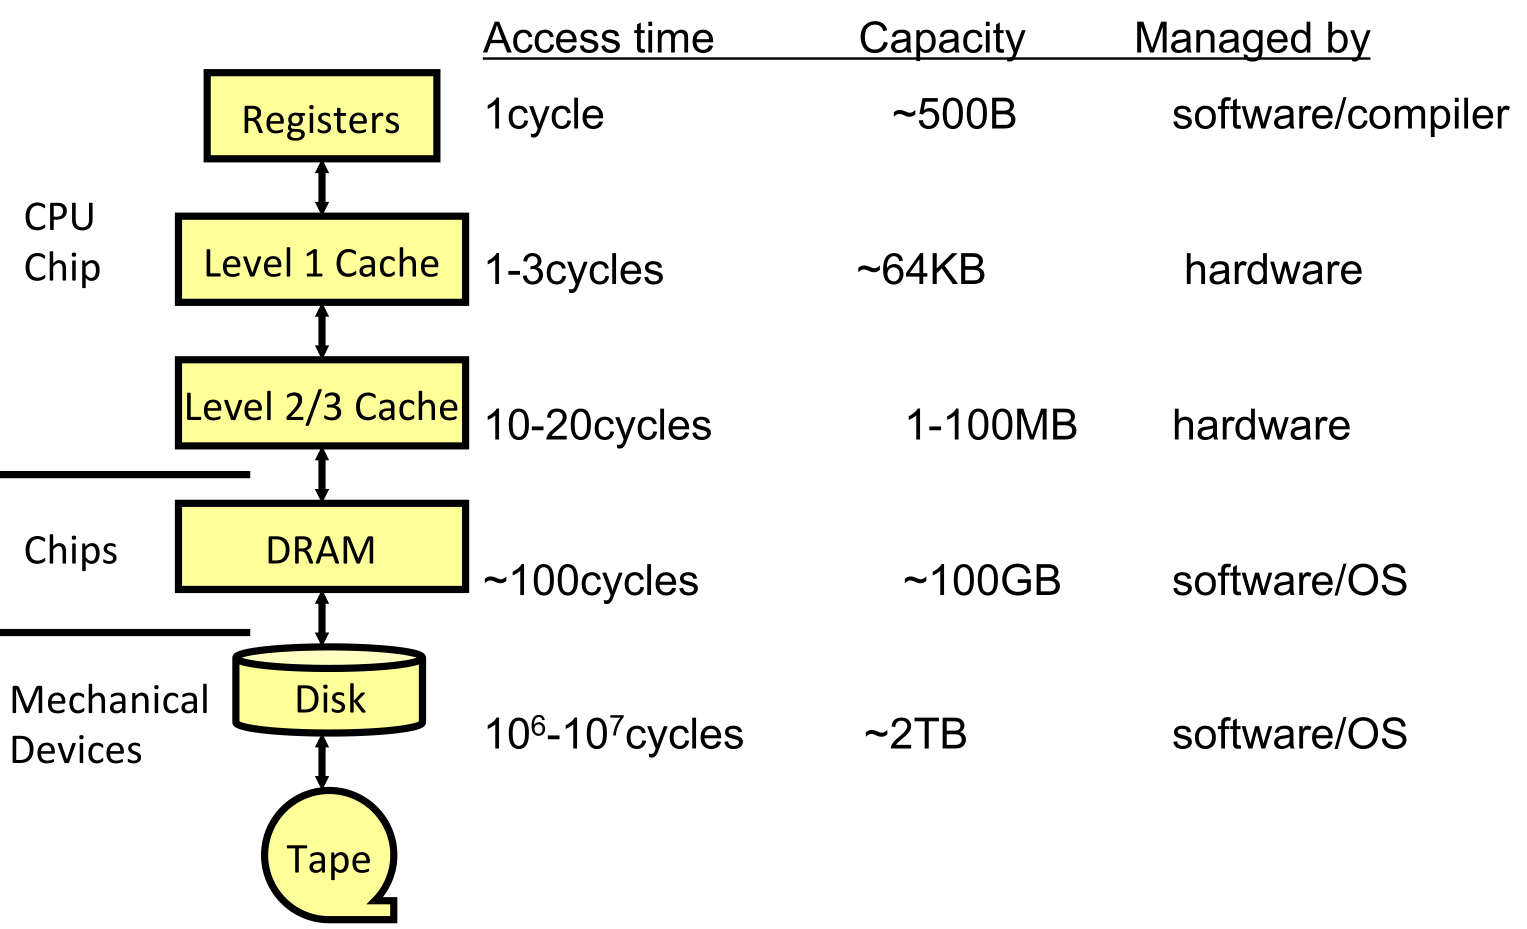
\includegraphics[width=\linewidth]{png/mem.png}
\textbf{Principle of locality} Programs work on a relatively small portion of data
at any time, so we can predict data accessed in near future by looking at recent accesses

There are two types of locality: \textbf{spatial} and \textbf{temporal},
\textbf{spatial} locality is if an item has been accessed recently, nearby items will tend to be
referenced soon, and \textbf{temporal} is if an item has been referenced recently,
it will probably be accessed again soon

How is data stored in a cache? There are three ways:
\begin{itemize}
\item Direct mapped (single location)
\item Fully associative (anywhere)
\item Set associative (anywhere in a set)
\end{itemize}

\subsection*{Direct Mapped Cache}
Location in cache determined by (main) memory address, we use the lowest order
bits to determine this address.

To determine which particular block is stored in a cache location, we look at
\textbf{tag} and \textbf{valid} bits, the \textbf{tag} bits are the high-order
bits of the memory address, the \textbf{valid} bit represents $1 =$ present,
$0 =$ not present
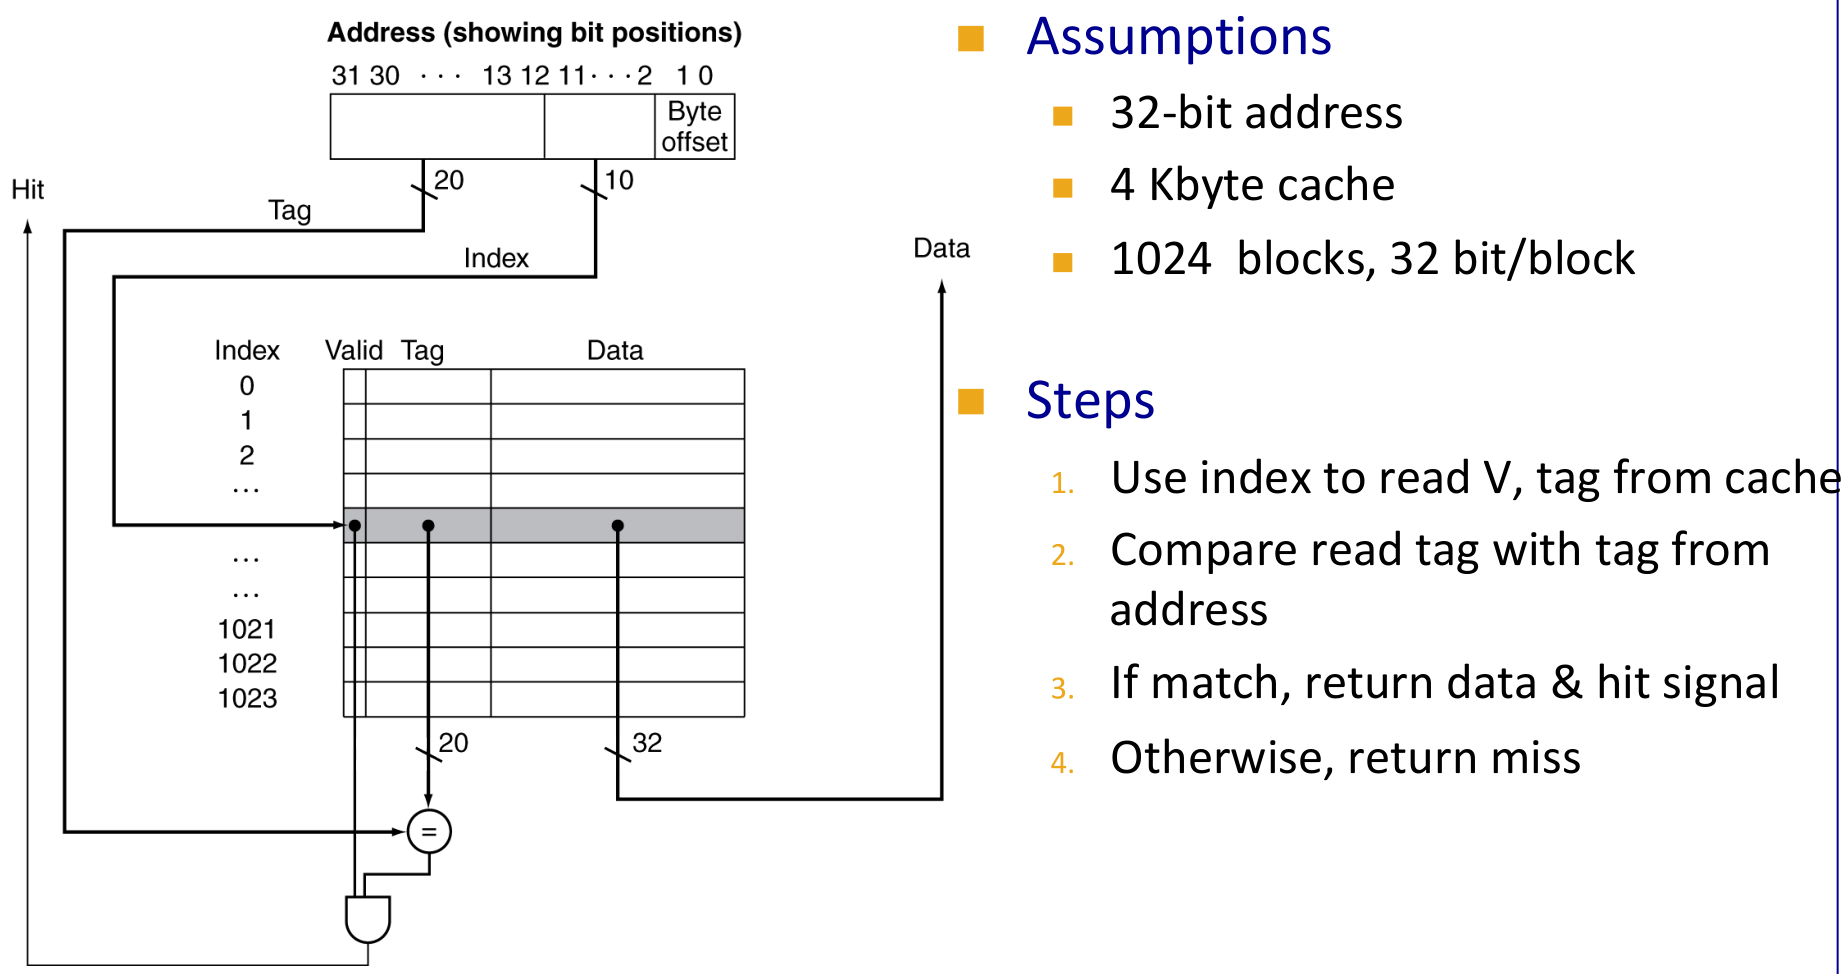
\includegraphics[width=\linewidth]{png/cache.png}
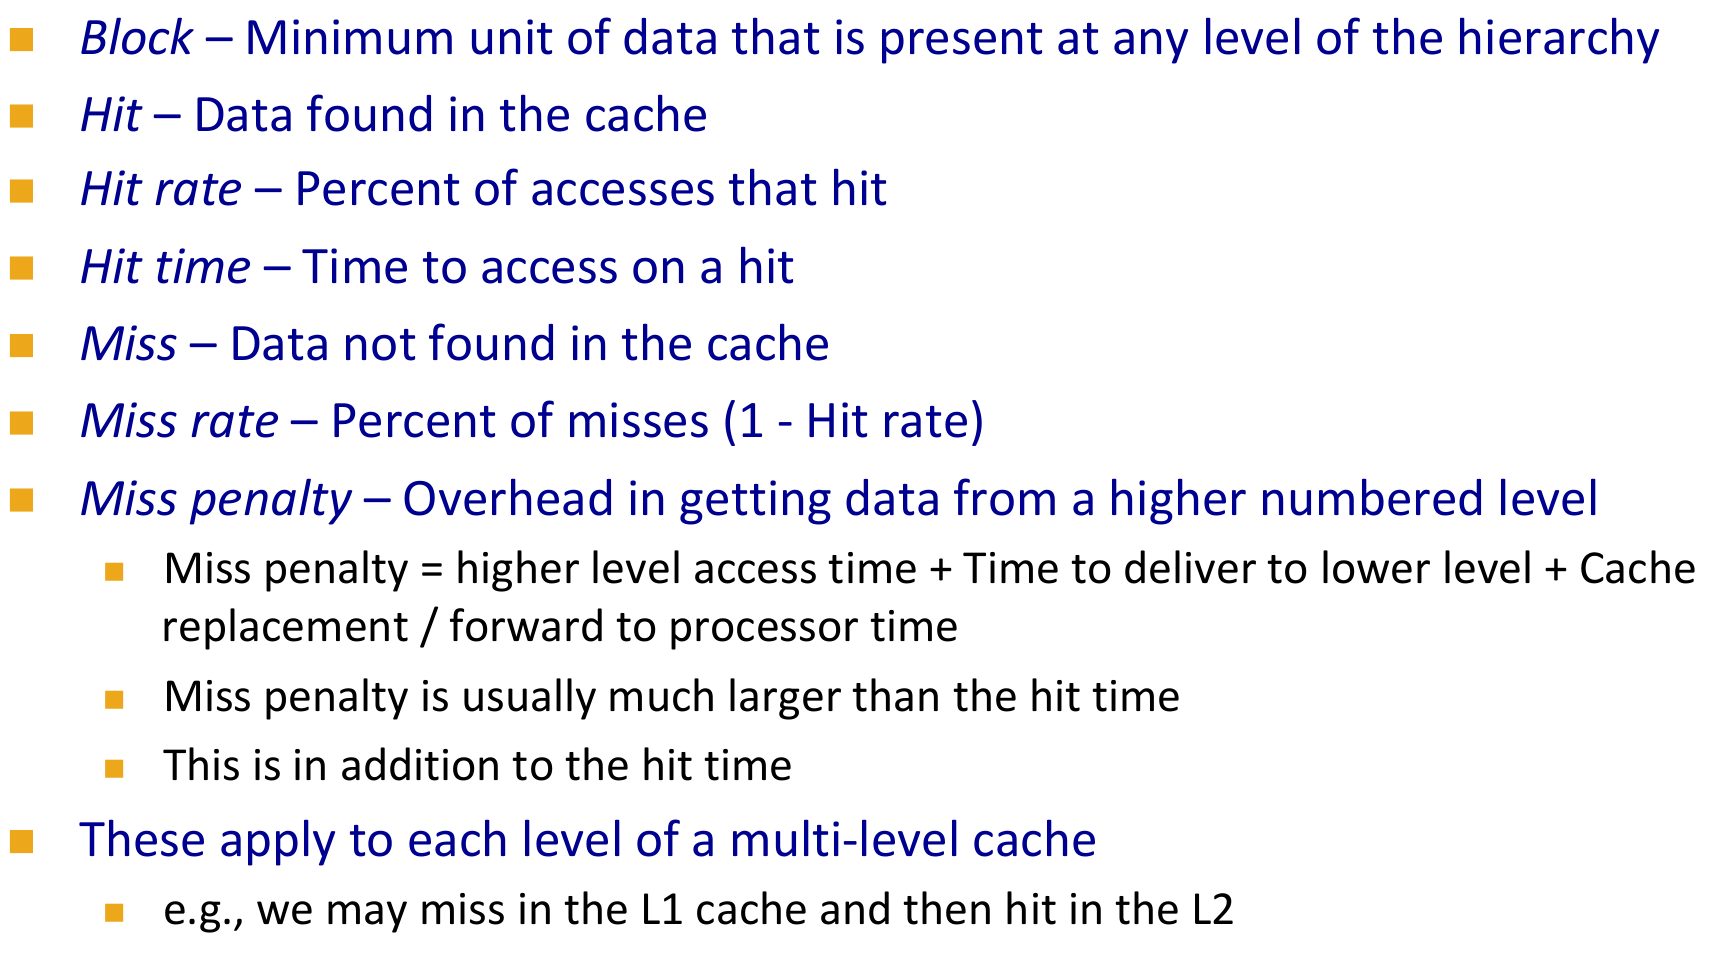
\includegraphics[width=\linewidth]{png/term.png}
\textbf{Average Memory Access Times}:

$Access time = hit time + miss rate \times miss penalty$

\textbf{3 C's of Cache Misses}:
\begin{itemize}
\item Compulsory – this is the first time you referenced this item
\item Capacity – not enough room in the cache to hold items
\par this miss would disappear if the cache were big enough
\item Conflict – item was replaced because of a conflict in its set
\par this miss would disappear with more associativity
\end{itemize}
$CPI penalty = miss rate \times miss penalty$

When we encounter a miss the pipeline stalls for an instruction or data miss \\

\subsection*{Cache Blocks}
Assuming a $2^n$byte direct mapped cache with $2^m$ byte blocks
\begin{itemize}
\item Byte select – The lower m bits
\item Cache index - The lower (n-m) bits of the memory address
\item Cache tag - The upper (32-n) bits of the memory address
\end{itemize}
Direct Mapped Problems: \textbf{Thrashing} If accesses alternate, one block will
replace the other before reuse

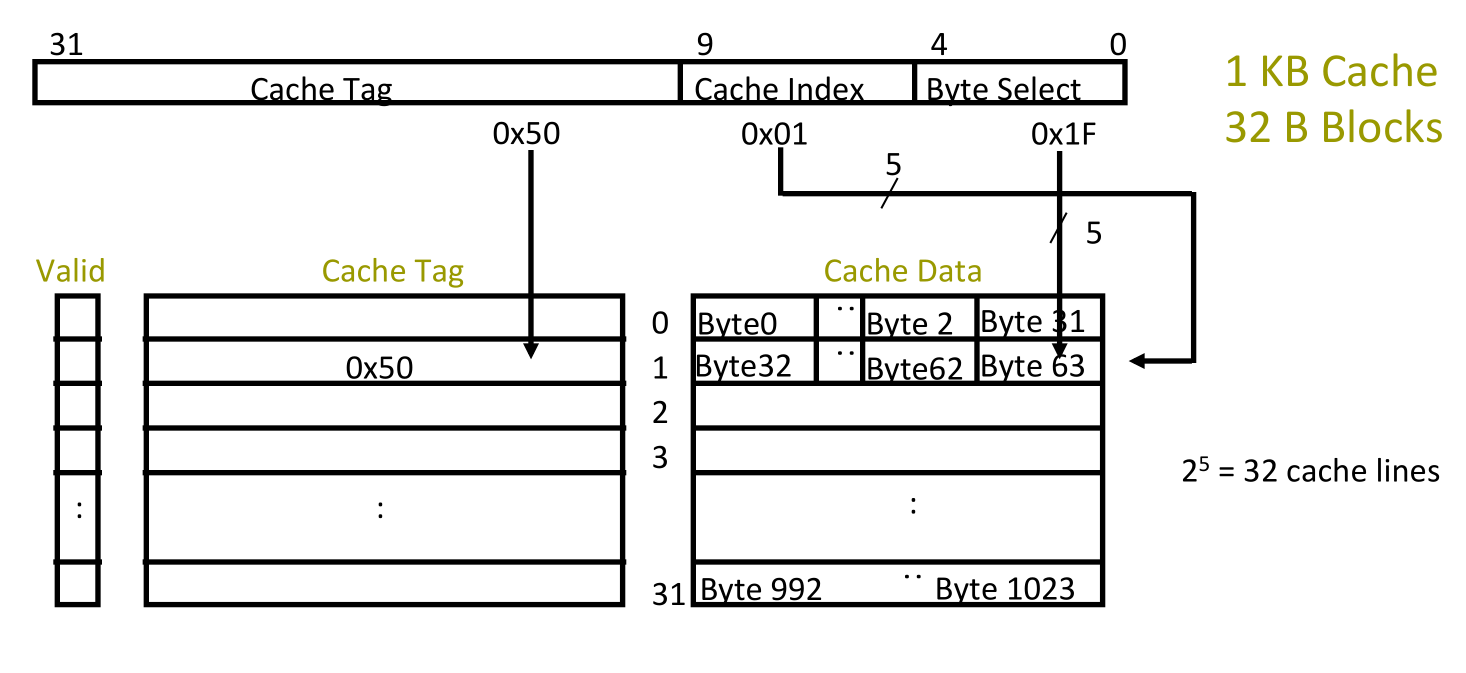
\includegraphics[width=\linewidth]{png/cacheblock.png}
\textbf{Block Sizes}: Larger block sizes take advantage of spatial locality,
however it also incurs larger miss penalty since it takes longer to transfer
the block into the cache.
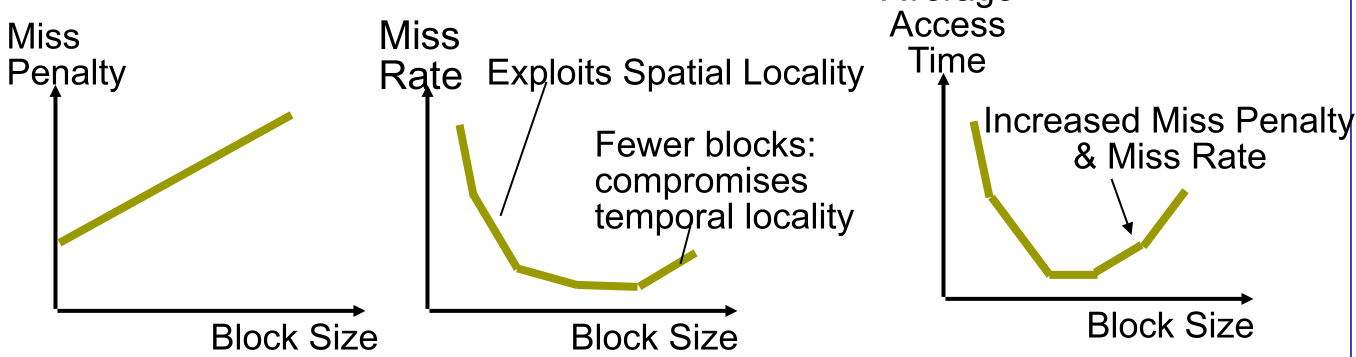
\includegraphics[width=\linewidth]{png/block.png}

\subsection*{Fully Associative Cache}
Opposite extreme in that it has no cache index to hash, it uses any available
entry to store memory elements, there are no conflict misses, only capacity
misses, and we must compare cache tags of all entries to find the desired one

%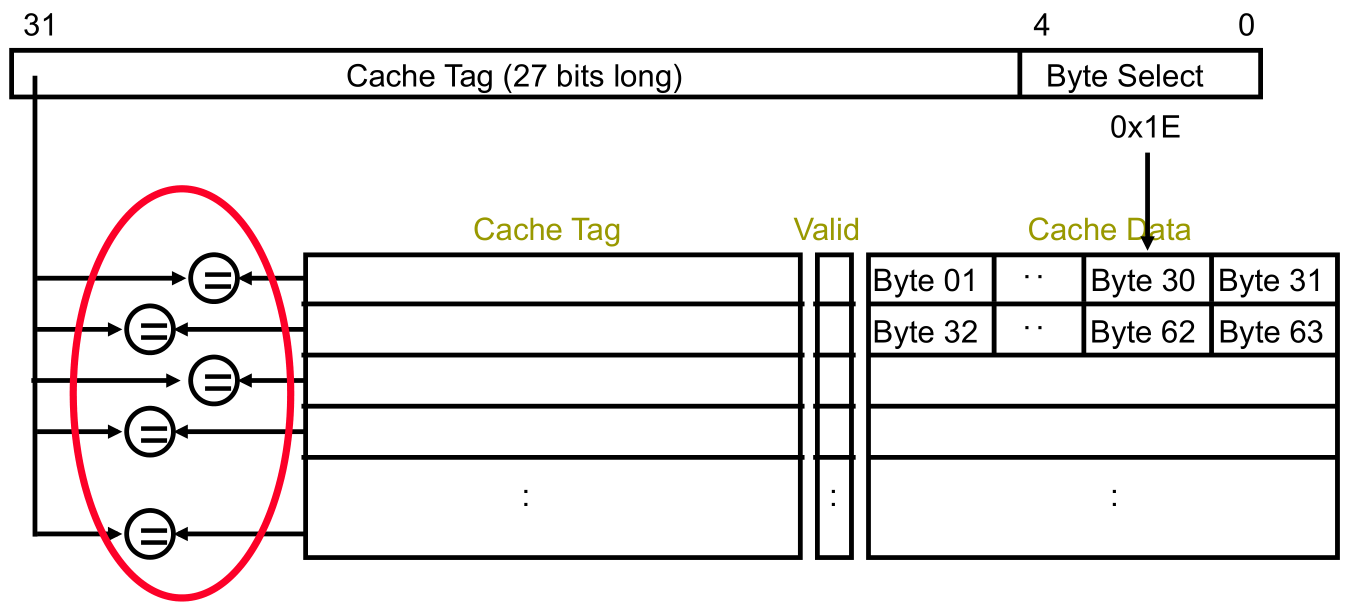
\includegraphics[width=\linewidth]{png/fully.png}

\subsection*{N-way Set Associative Cache}
Compromise between direct-mapped and fully associative, each memory block can go
 to one of N entries in cache, and each set can store N blocks; a cache contains
 some number of sets
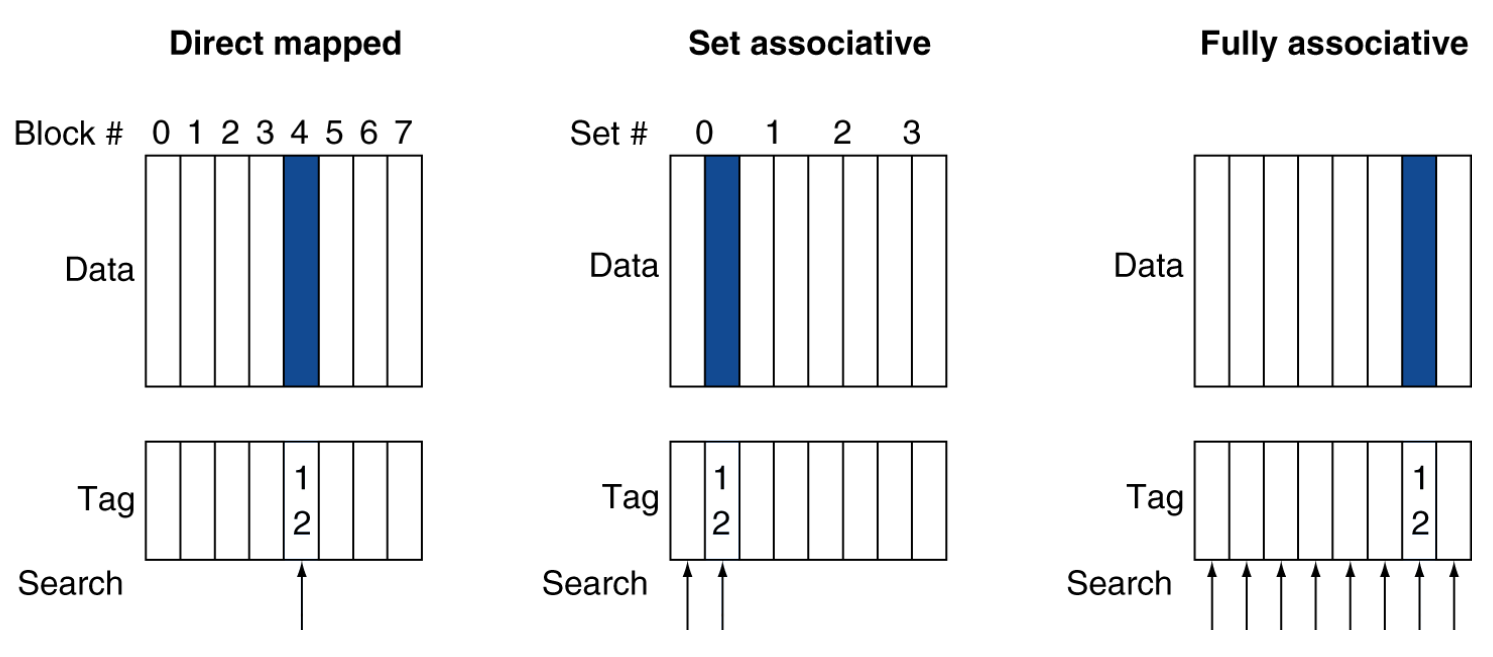
\includegraphics[width=\linewidth]{png/nway.png}

\subsection*{Tag \& Index with Set-Associative Caches}
Given a $2^n$ byte cache with $2^m$ byte blocks that is $2^a$ set-associative,
the cache contains $2^{n-m}$ blocks, and each cache way contains $2^{n-m-a}$ blocks,
and the cache index is $n-m-a$ bits after the byte select

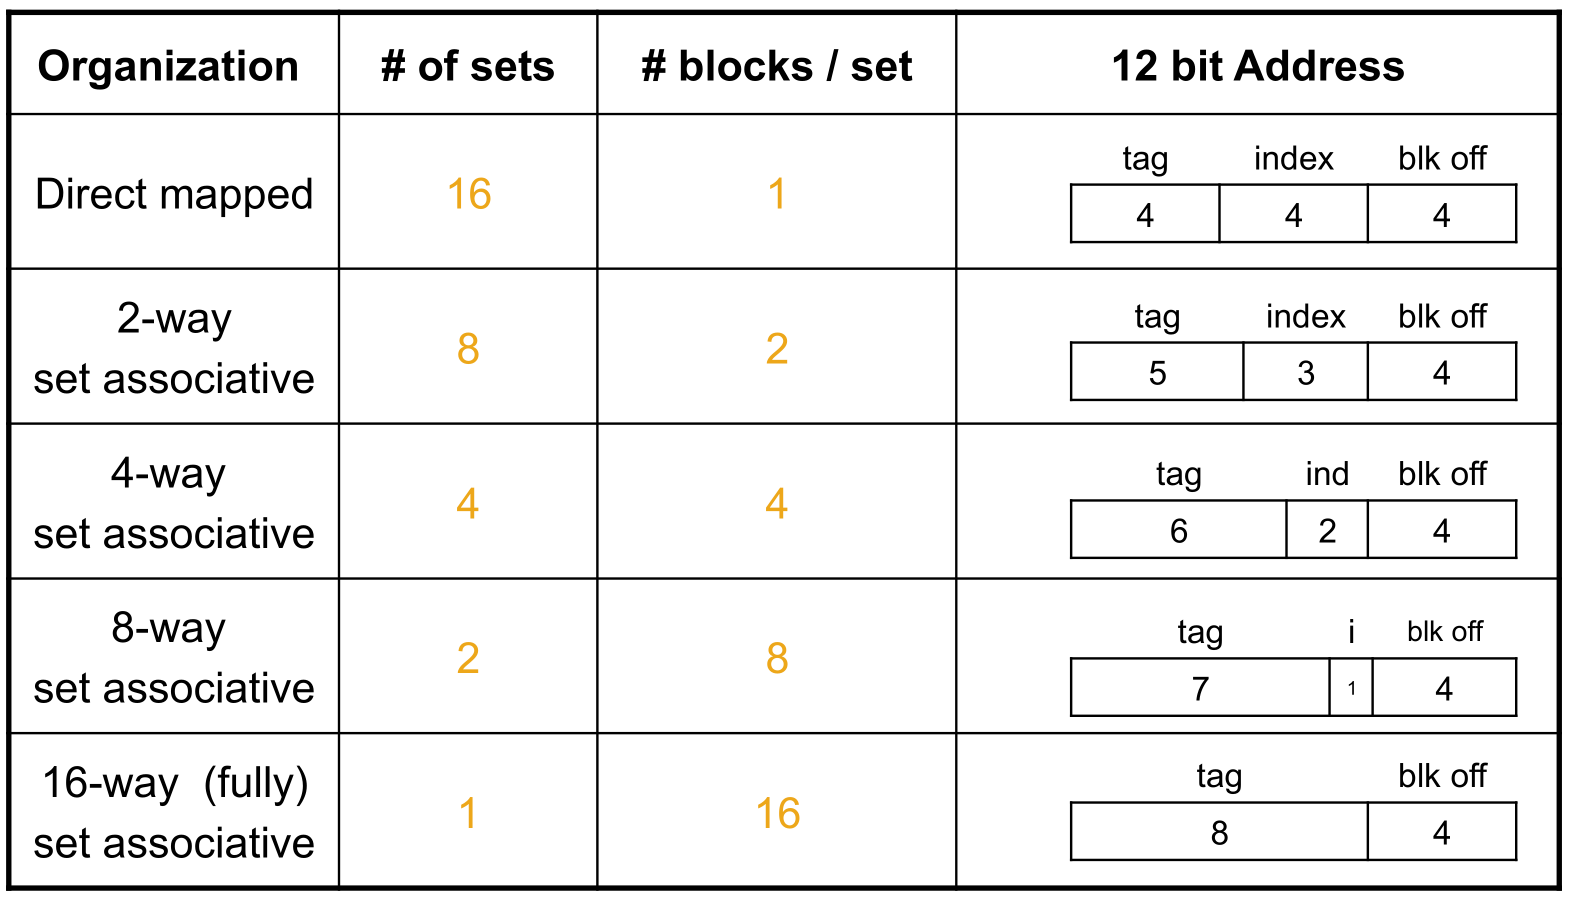
\includegraphics[width=\linewidth]{png/ex.png}
Some cons with associative caches are that there is an an area overhead and more latency

The \textbf{replacement policy} for a N-way set associative cacheis choosing the
least recently used thing

\subsection*{Cache Write Policies}
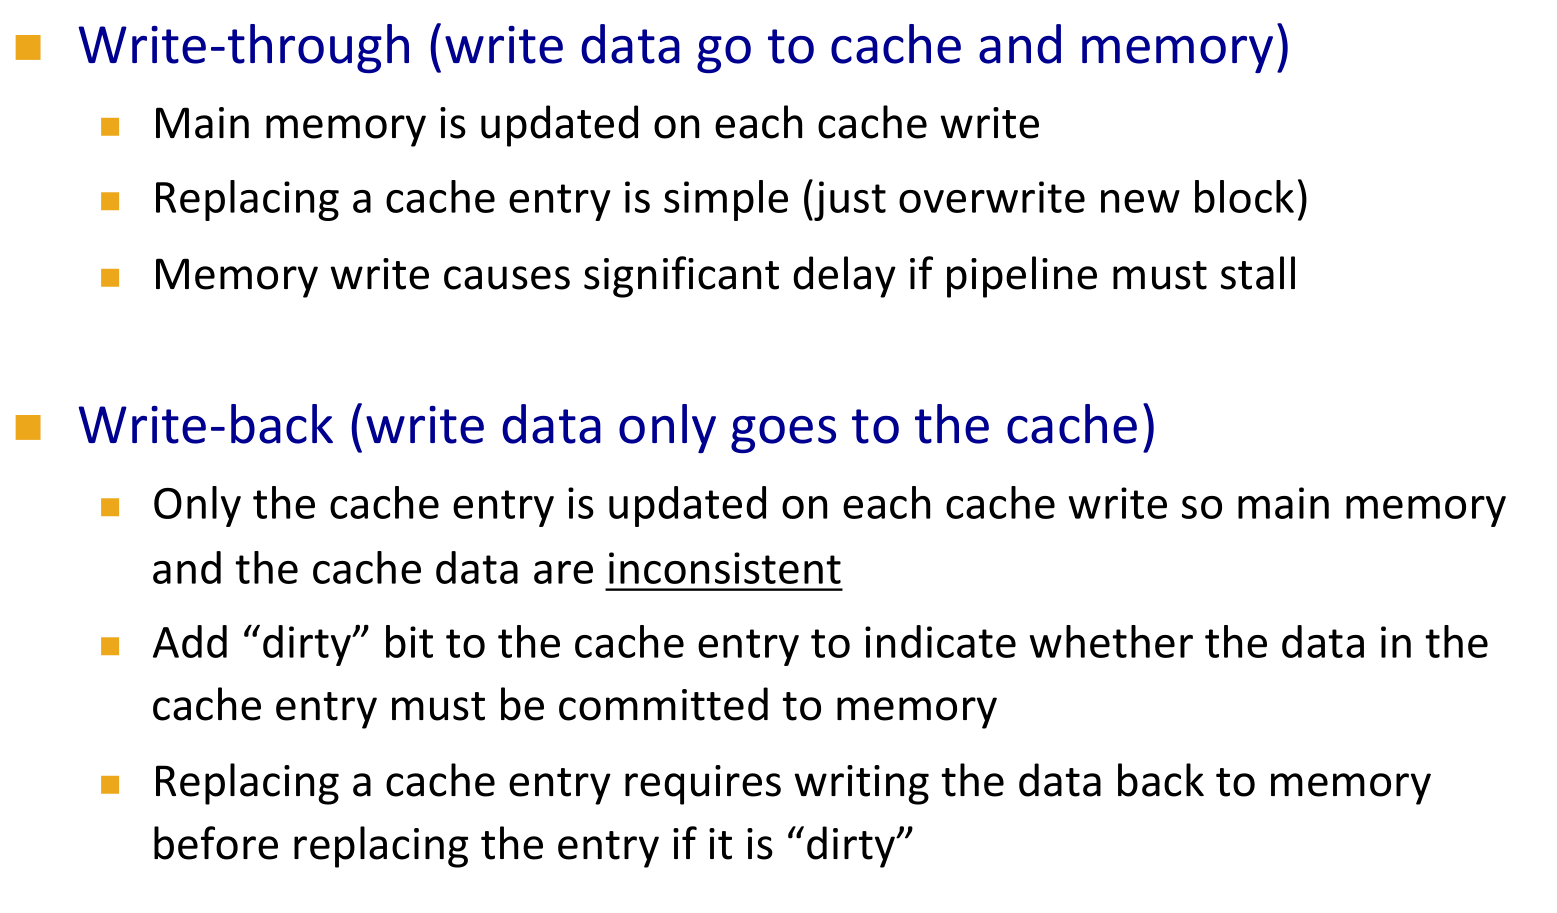
\includegraphics[width=\linewidth]{png/write.png}
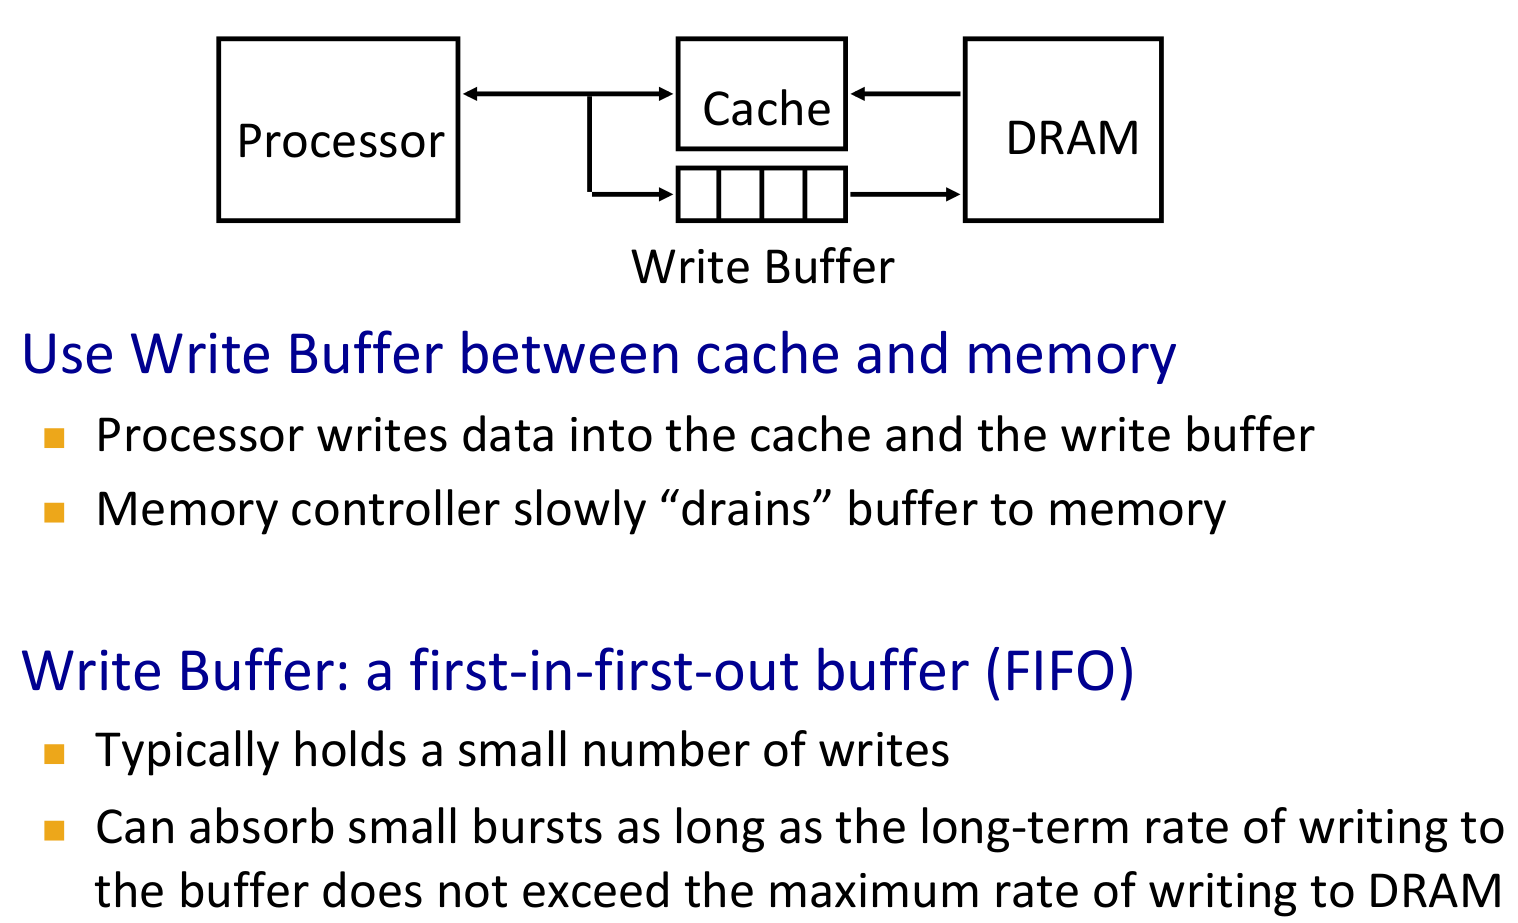
\includegraphics[width=\linewidth]{png/write(1).png}
\textbf{Write Miss Options}:

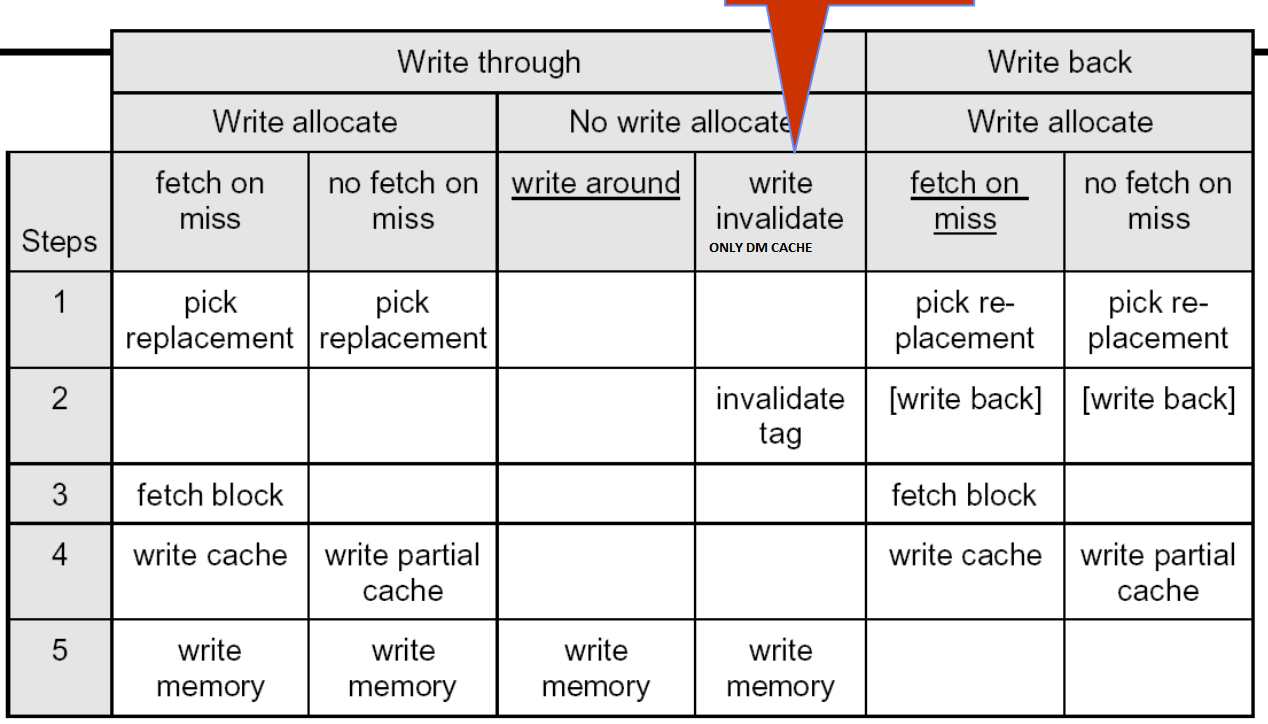
\includegraphics[width=\linewidth]{png/writemiss.png}

\textbf{Splitting Caches} Most chips have separate caches for instructions and
data, some advantages are that we have extra bandwidth and low hit time, but miss
rate will be higher.

\textbf{Multilevel Caches:} Different levels of caches L1, L2, and L3. L1 is focused
on hit time L2 is focused on hit rate, L3 is extra.

\textbf{Cache Coherence:} State and sequence of actions needed to ensure caches
are coherence in multi-core systems, there are protocols that rely on monitoring
other caches.

\textbf{MSI Coherence Protocol}

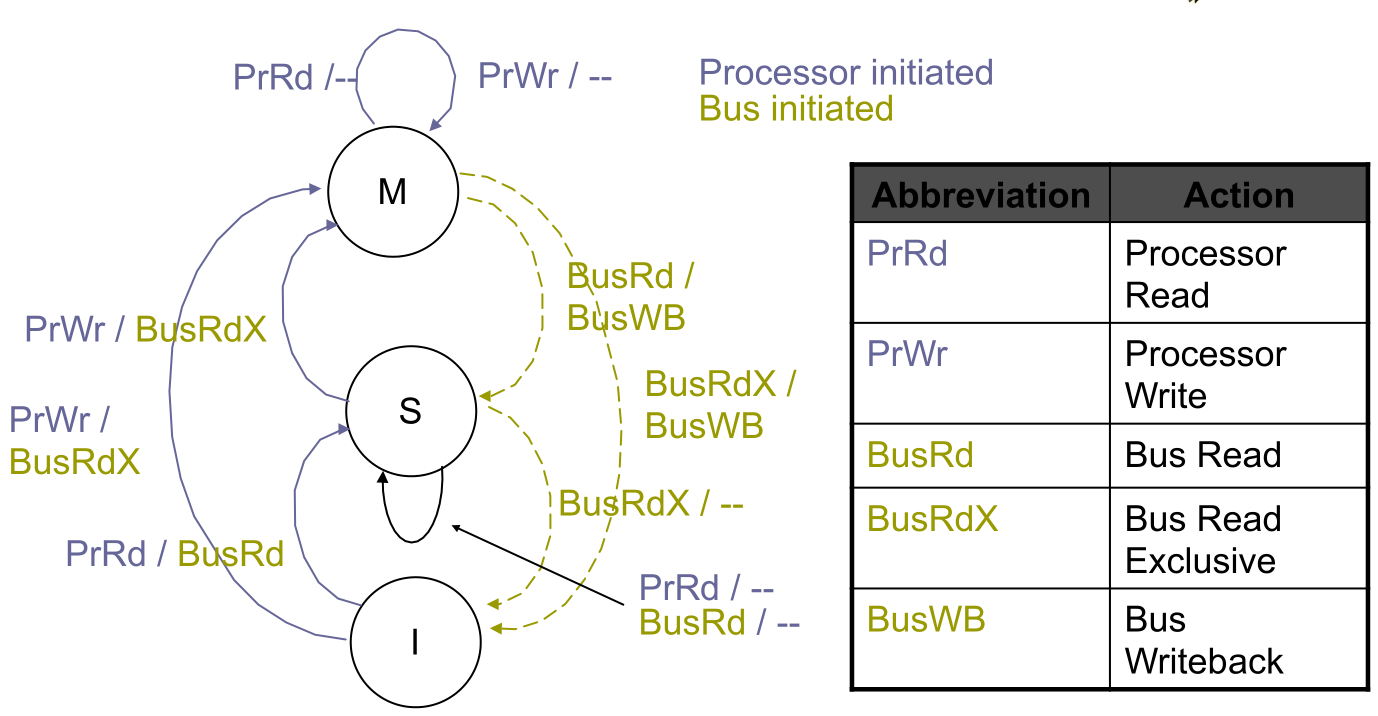
\includegraphics[width=\linewidth]{png/msi.png}

\vfill\null
